\documentclass{scrartcl}
\usepackage{amsmath,amsfonts,amsthm,bm,graphicx}
\usepackage{tikz,pgfplots}
\usepackage{listings}
\usepackage{stmaryrd}
\usepackage{xcolor}
\usepackage{rotating}
\usepackage{listings}
\usepackage{hyperref}

\pgfplotsset{width=15cm,compat=1.18}
\allowdisplaybreaks
\setlength{\parindent}{0pt}

\title{Assignment 5}
\subtitle{Angewandte Modellierung 25}
\author{Carl Colmant}
\date{\today}
\begin{document}
\maketitle
\newpage
\section*{Exercise 1. Poisson equation}
Mit der Poisson Gleichung will man eine Funktion f approximieren. In unserem Fall lösen wir die Gleichung für den Einheitskreis.\\
\subsection*{a)}
Ich habe die funktion $f(x,y) = sin^2(x^2+y^2)$ gewählt.\\
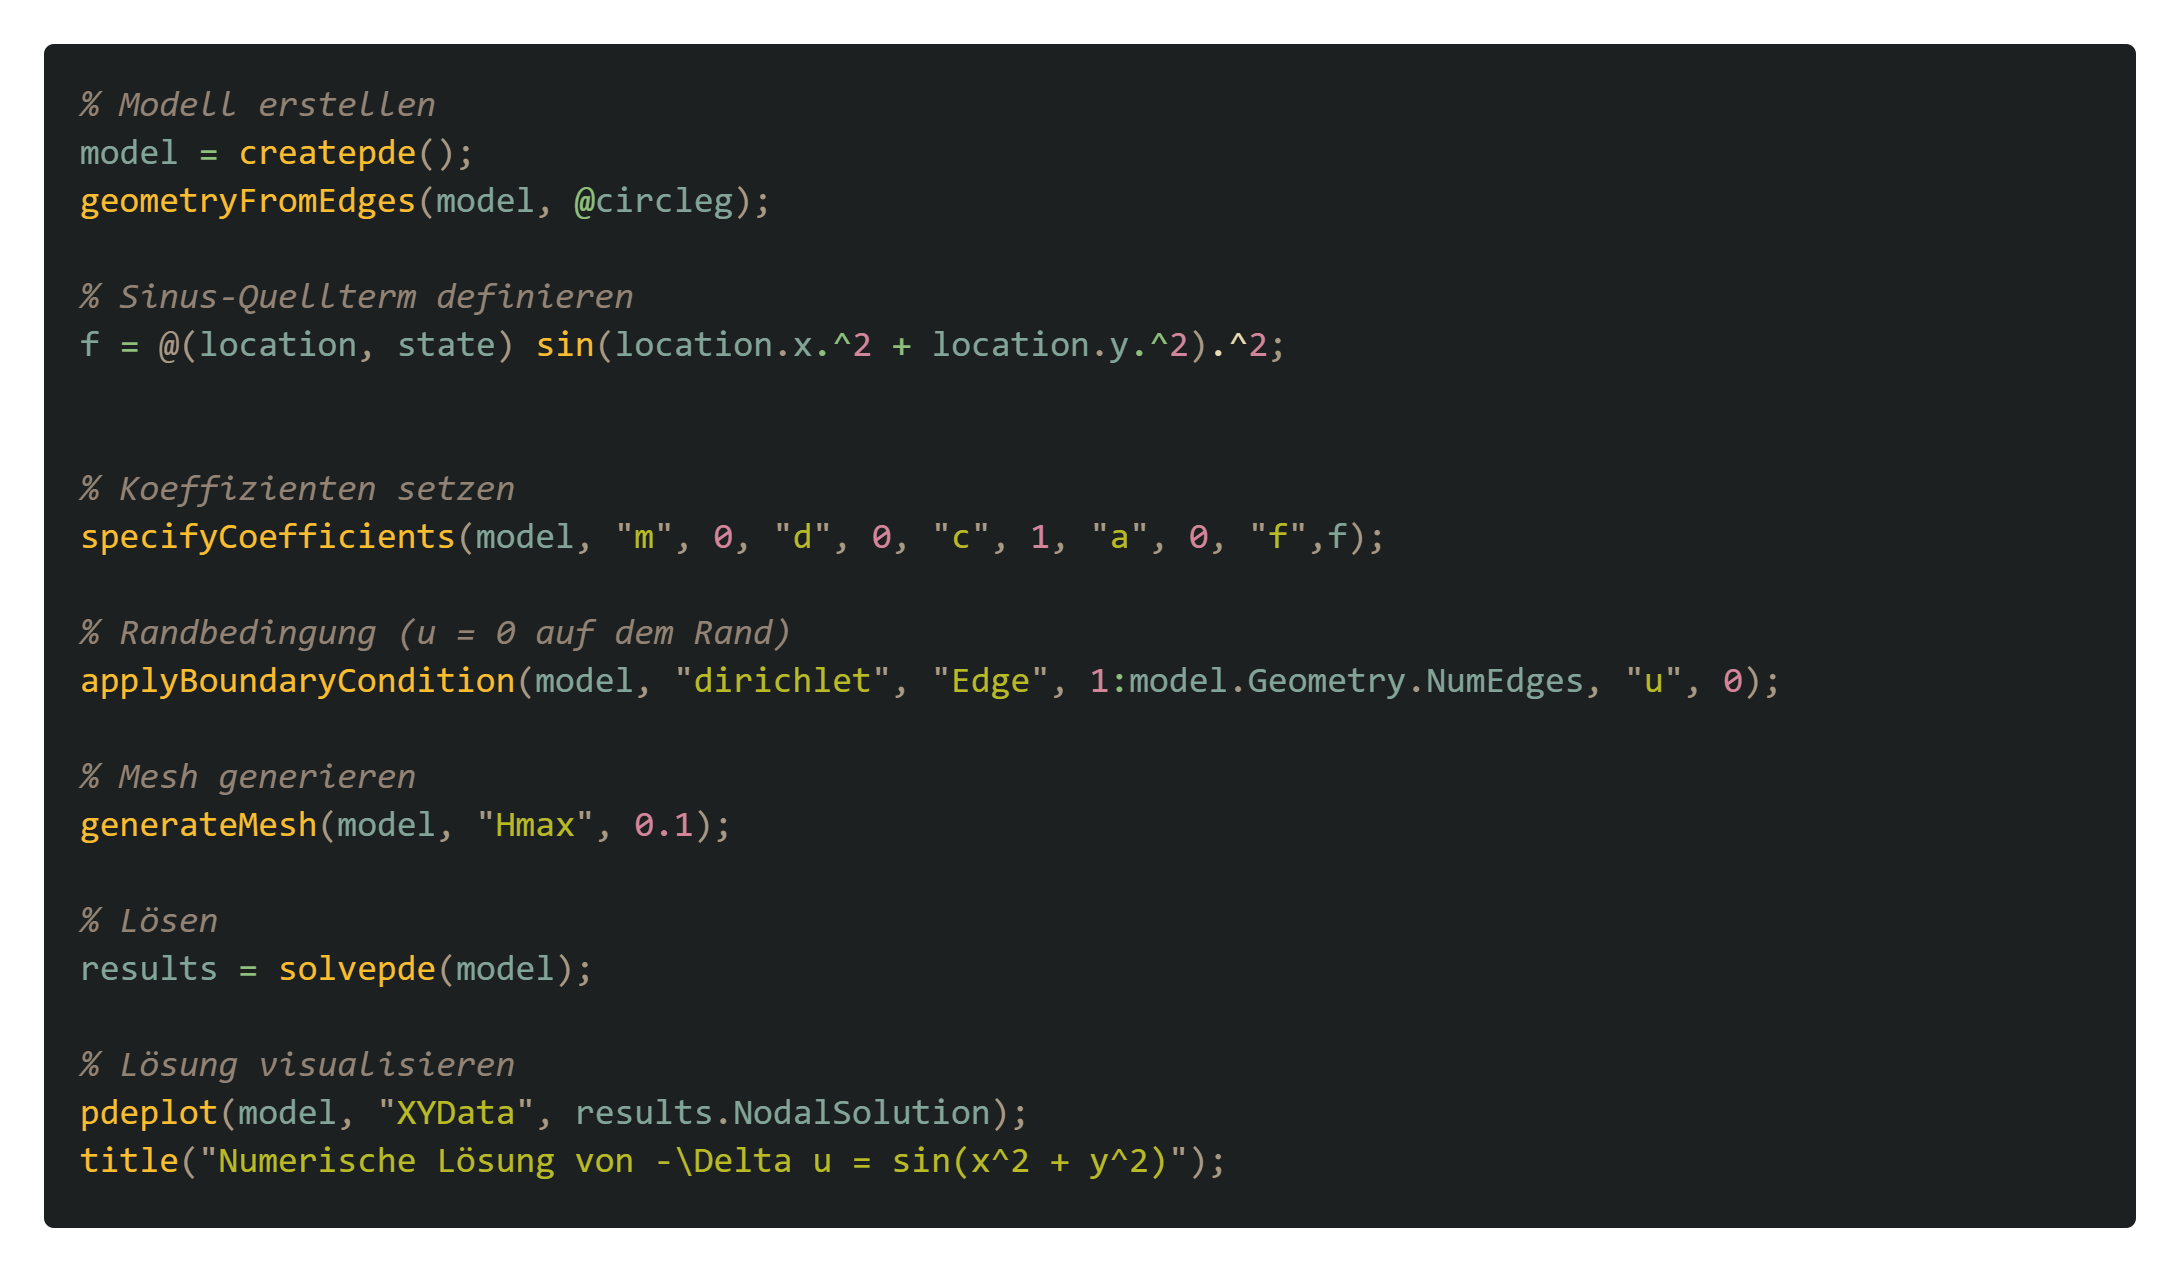
\includegraphics[scale=0.2]{Poisson1a.png}\\
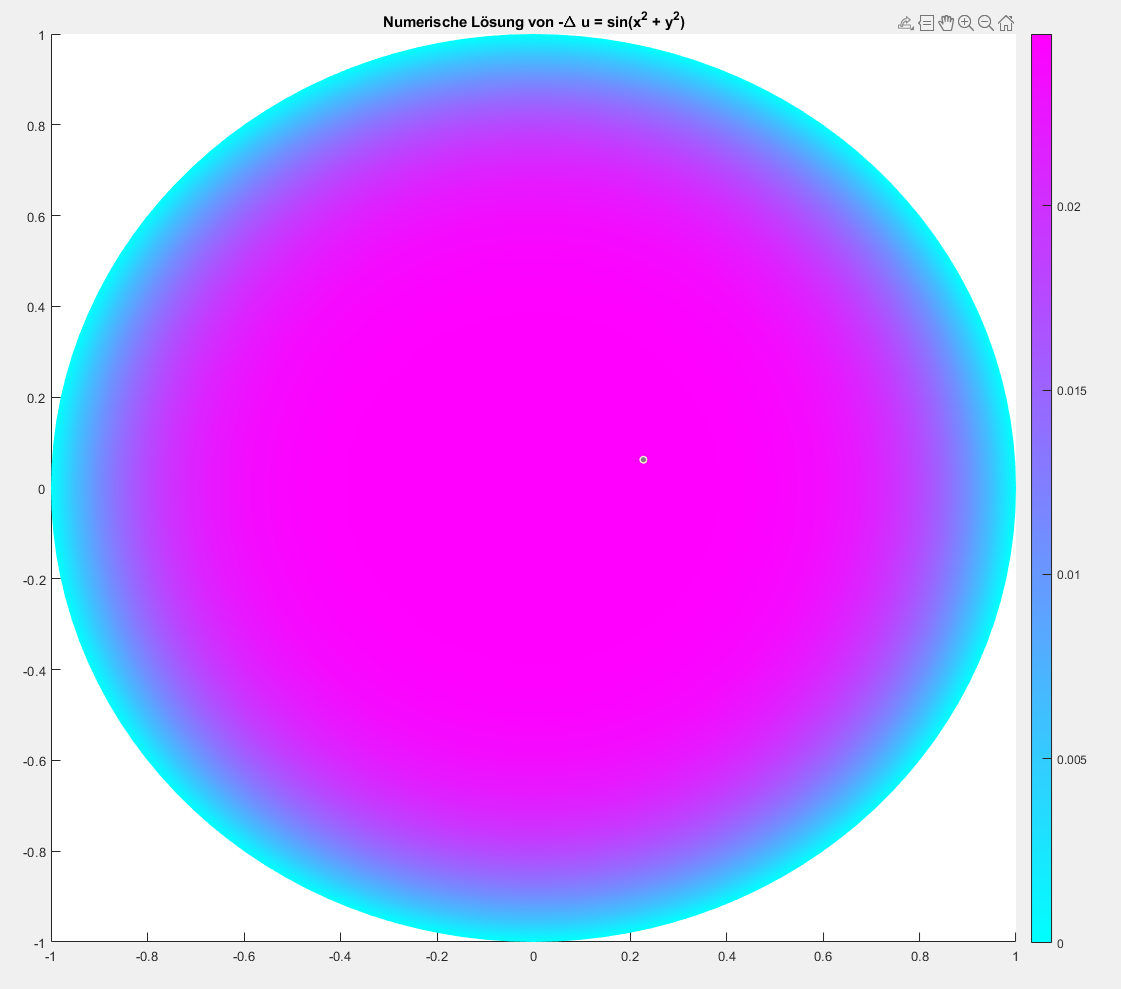
\includegraphics[scale=0.4]{Poisson1aplot.png}\\
Im Gegensatz dazu, die Funktion $f(x,y) = 1$ also der Einheitskreis:\\
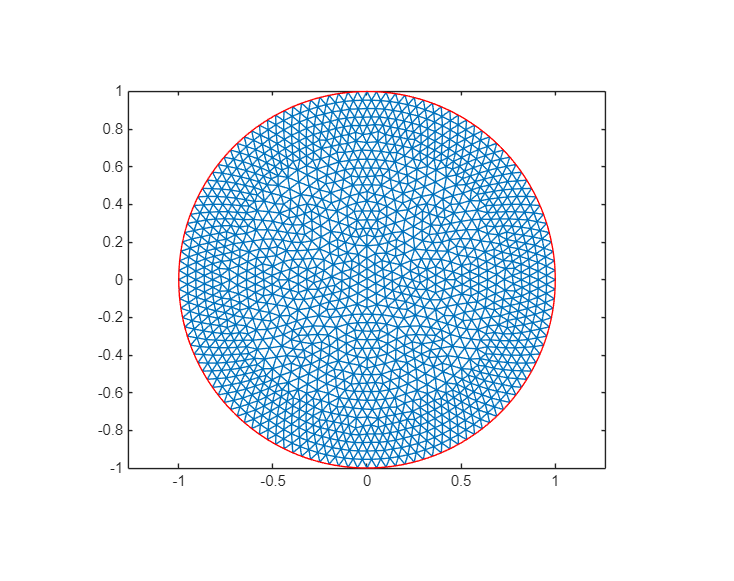
\includegraphics[scale=0.5]{Poisson1aplot2mesh.png}
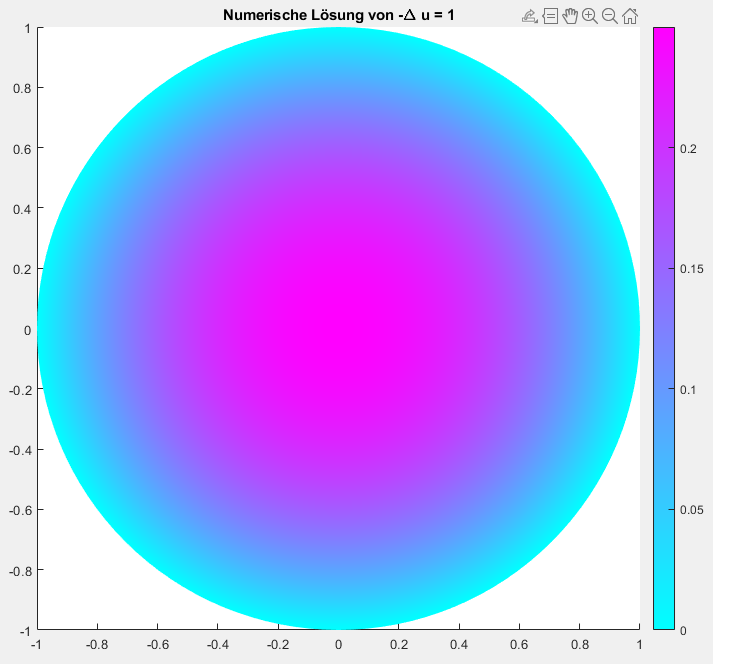
\includegraphics[scale=0.4]{Poisson1aplot2.png}\\
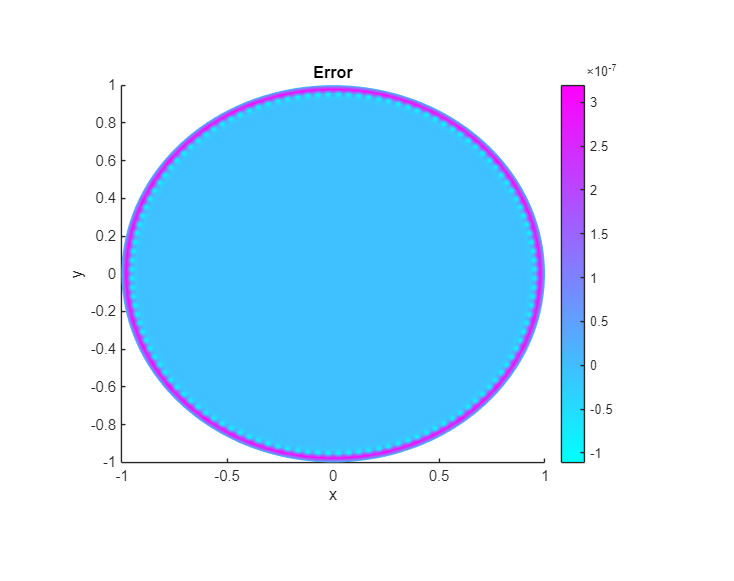
\includegraphics[scale=0.7]{Poisson1aplot2error.png}\\


\subsection*{b)}
Im gegensatz zu a) benutzt der pde Modeler eine andere Funktion zur berechnung des Meshes und somit entsteht eine etwas andere Lösung. Dies kann nur im Error gesehen werden also im Vergleich der Perfekten Lösung.\\
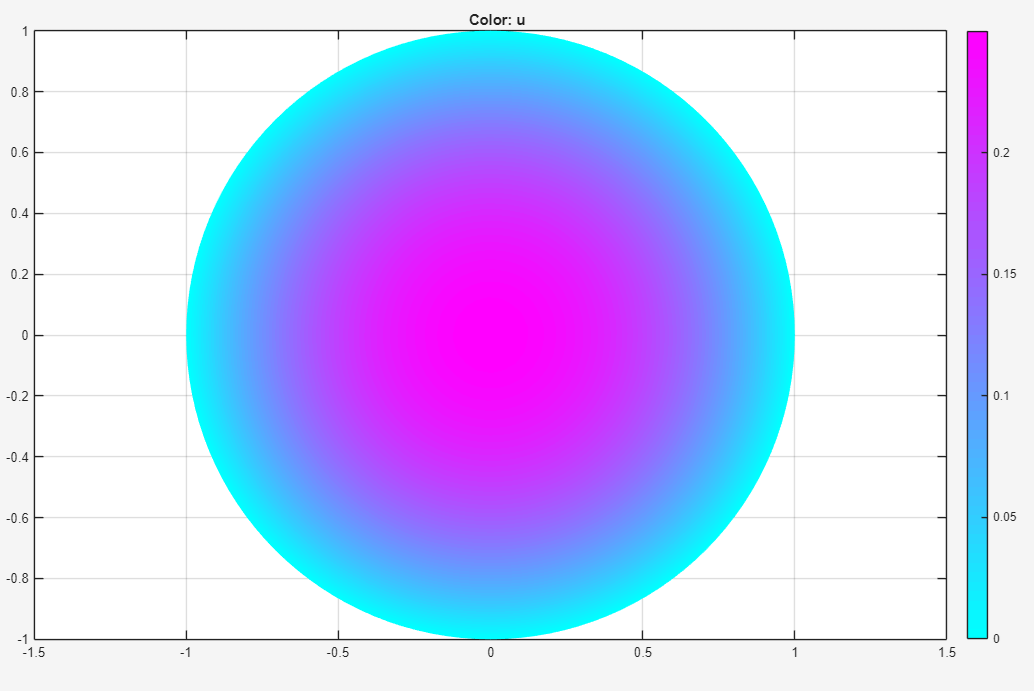
\includegraphics[scale=0.5]{Poisson1bplot.png}\\
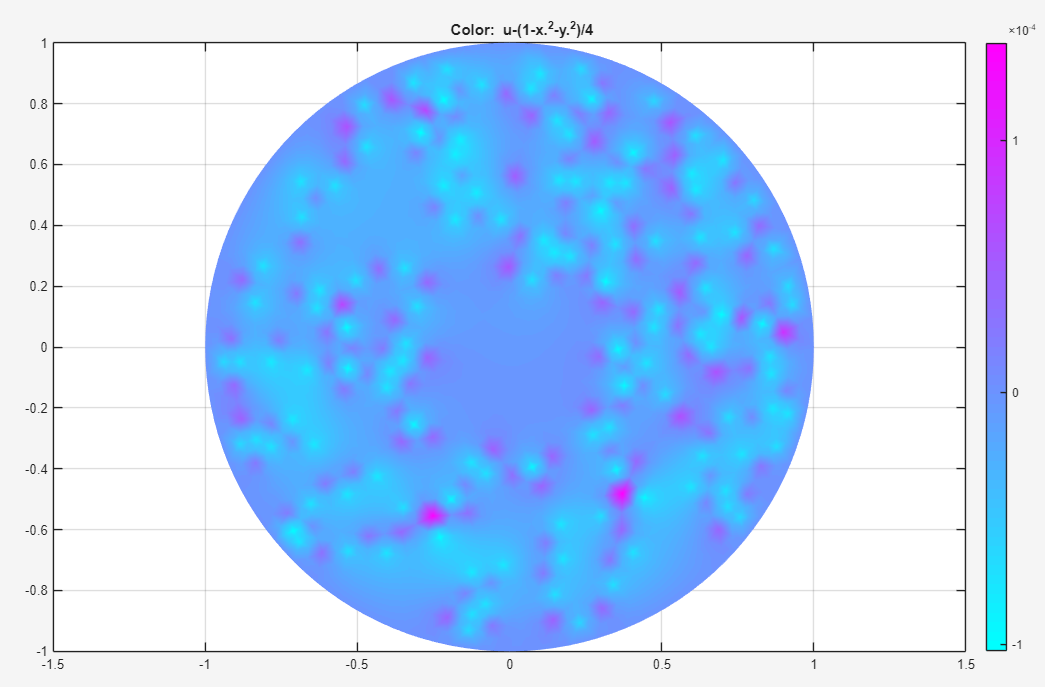
\includegraphics[scale=0.3]{Poisson1aplotERROR.png}
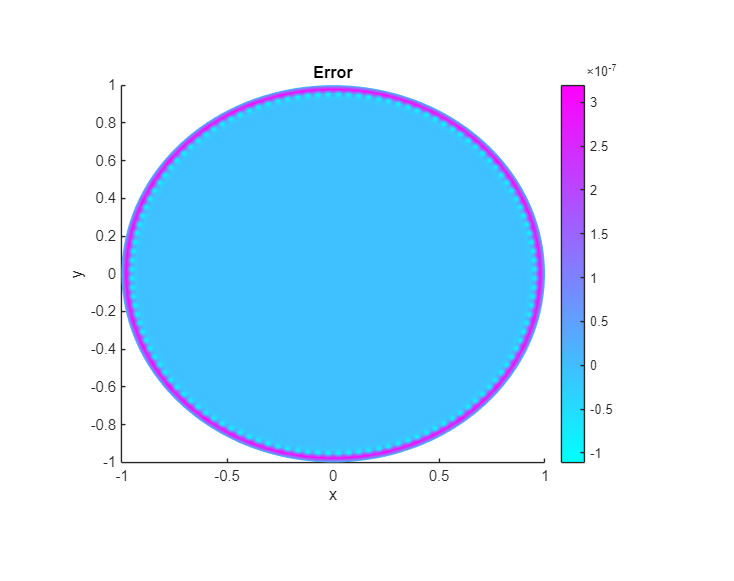
\includegraphics[scale=0.4]{Poisson1aplot2error.png}\\

Wenn man beide Error plots gegenüber stellt sieht man das bei der Implementation aus dem Livescript die Fehler aussen am Kreis sich verteilen wehrend die Fehler bei der Implementation aus dem PDE Modeler sich eher im Kreis verteilen.\\

\section*{Exercise 2. Helmholtz's equation}
Die Helmholtz Gleichung ist:\\
\begin{equation*}
    \nabla\times \left(\frac1{\mu_r}\nabla\times E\right)- k_0^2\left(\epsilon_r-j\frac{\sigma}{\omega\epsilon_0}\right)E = 0
\end{equation*} wobei
\begin{itemize}
    \item E: elektrische Feld
    \item $\nabla$ ist die Ableitung nach dem ort
    \item $\mu_r$: relative Permeabilität in dem Script ist $\mu_r = 1$
    \item $\epsilon_r$: relative Permittivität in dem Script ist $\epsilon_r = 1$
    \item $\sigma$: elektrische Leitfähigkeit in dem Script ist $\sigma = 0$
    \item $\omega$: Frequenz in dem Script ist $\omega = 4\pi$
    \item $\epsilon_0$: elektrische Feldkonstante in dem Script ist $\epsilon_0 = 1$
    \item $\mu_0$: magnetische Feldkonstante in dem Script ist $\mu_0 = 1$
    \item k: Wellenzahl in dem Script ist $k = \frac{\omega}{c} = \frac{\omega}{\sqrt{\mu_0\epsilon_0}}$
\end{itemize}
Das ist eine imaginäre Funktion.\\
\subsection*{a)}
wenn wir die schritte des Demo files folgen bekommen wir folgenden plot:\\
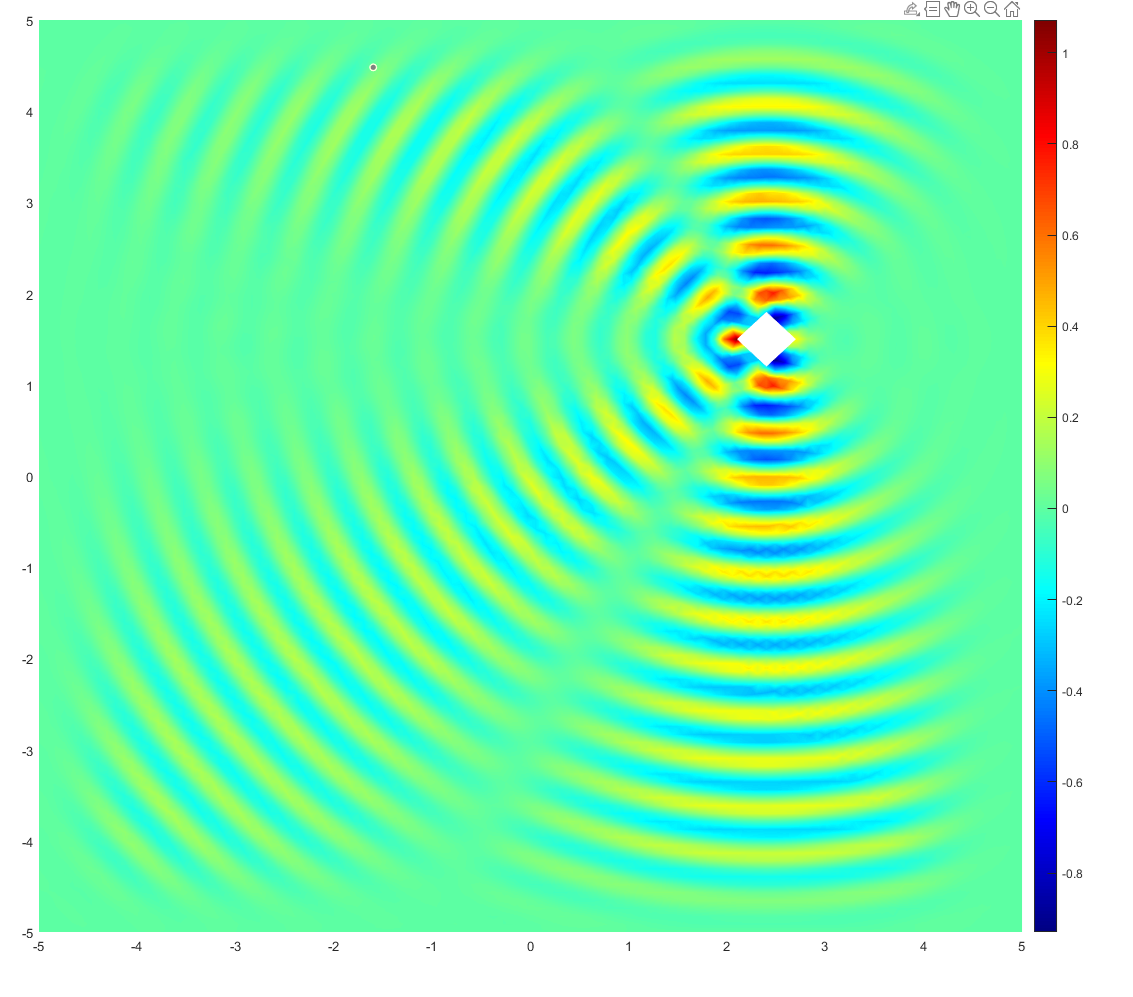
\includegraphics[scale=0.5]{Helmholzplot.png}\\
\subsubsection{b)}
Um das Ergebnis mit dem PDE Modeler zu erhalten müssen wir einmal das Rechteck als äussere Einschränkung definieren dazu setzten wir im PDE Modeler die boundary conditions im Neumann modus auf $g=0$ und $q=-i*4*pi$ und für die eingezeichnete Raute im Dietrich modus auf $h = 1$ und $r = -e^{-i*4*pi*x}$. Nun muss noch die differential gleichung die approximiert werden soll in das system gegeben werden. Dazu müssen wir die Helmholtz Gleichung in eliptischer Form unter PDE specification definieren. Dazu setzen wir $c =1,f=0$ und $a=-(4*pi)^2$. Aus diesen Einstellungen erhalten wir folgenden Polt:\\
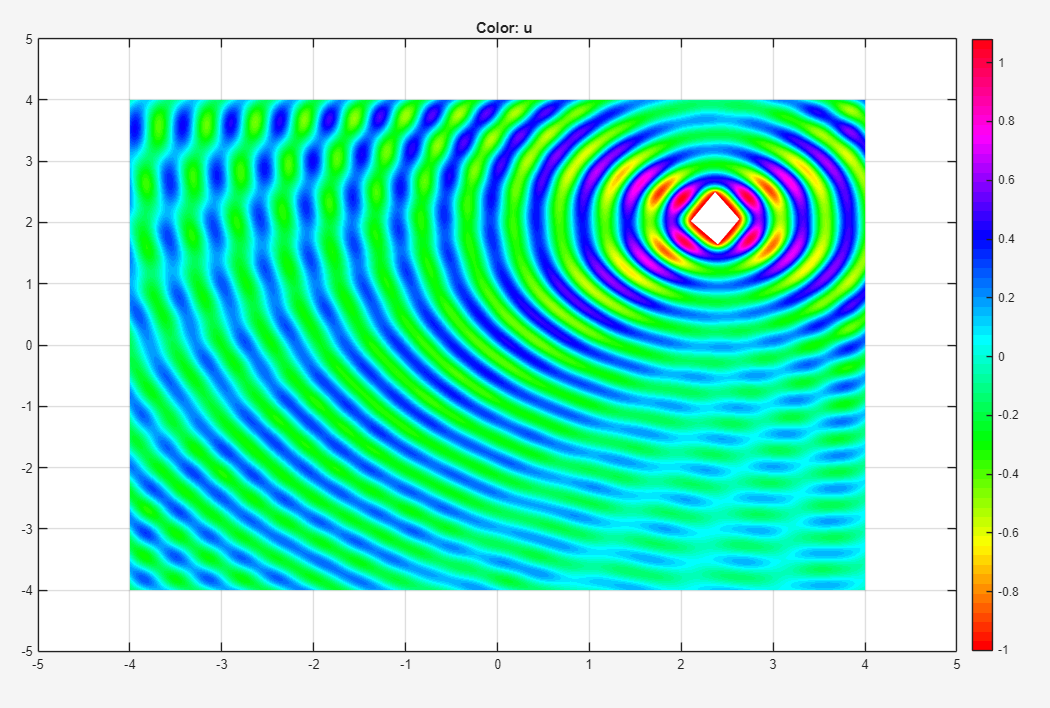
\includegraphics[scale=0.6]{Helmholzplotmodeler.png}\\
Ich habe nur ein Quadrat von -4 bis 4 geplottet, sonst ist das Ergebnis aber sehr ähnlich.\\
\section*{Exercise 3. Heat equation}
disclaimer: heavy AI usage.
\subsection*{1. Inhomogeneous Heat Equation on Square Domain (`pdedemo5`)}

\textbf{Gleichung:}
\[
\frac{\partial u}{\partial t} \;-\;\Delta u \;=\;1
\quad\text{auf dem Quadrat } \{-1 \le x,y \le +1\}
\]
mit einer kreisförmigen Aussparung \(x^2+y^2 \le 0.4^2\).

\medskip
\textbf{Anfangsbedingung:}
\[
u(x,y,0) =
\begin{cases}
1, & \text{falls }x^2+y^2 \le 0.4^2,\\
0, & \text{sonst.}
\end{cases}
\]

\medskip
\textbf{Randbedingungen:}
\[
u(x,y,t) \;=\; 0
\quad\text{für alle Punkte an den vier Seiten des Quadrats.}
\]

\bigskip
\subsection*{2. 1D Heat Equation mit \texttt{pdepe} (Beispiel 1)}

\textbf{Gleichung:}
\[
\pi^2 \,\frac{\partial u}{\partial t}
\;=\;
\frac{\partial^2 u}{\partial x^2},
\quad 0 \le x \le 1.
\]

\medskip
\textbf{Anfangsbedingung:}
\[
u(x,0) = \sin(\pi x).
\]

\medskip
\textbf{Randbedingungen:}
\[
\begin{aligned}
&u(0,t) = 0,               &&\text{(homogene Dirichlet)}\\
&\frac{\partial u}{\partial x}(1,t)
  = -\pi\,e^{-t},          &&\text{(inhomogene Neumann)}.
\end{aligned}
\]
\subsection*{diffusion equation}
\section*{Lösung der Diffusionsgleichung mit implizitem Euler}

Wir betrachten
\[
\frac{\partial u}{\partial t}
= D\,\frac{\partial^2 u}{\partial x^2},
\quad x\in[0,1],\ t\in[0,T],
\]
mit
\[
D = 0.01,\quad
u(x,0) = \exp\bigl(-100(x-0.5)^2\bigr),\quad
u(0,t)=u(1,t)=0.
\]

\subsection*{Diskretisierung}
\begin{itemize}
  \item Raumgitter: $N_x=51$ Punkte, \quad $\Delta x = \tfrac{1}{N_x-1}=0.02$.
  \item Zeitschritte: $N_t=200$, \quad $\Delta t = T/N_t=0.2/200=0.001$.
  \item Implizites Euler: 
    \[
      \mathbf{A}\,\mathbf{u}^{\,n+1}
      = \mathbf{u}^{\,n},
    \]
    wobei nur die inneren Gitterpunkte $i=2,\dots,N_x-1$ betrachtet werden.
\end{itemize}

\subsection*{Matrixaufbau}
Setze $N=N_x-2$ und
\[
\alpha = \frac{D\,\Delta t}{(\Delta x)^2}.
\]
Dann ist $\mathbf{A}\in\mathbb{R}^{N\times N}$ tridiagonal mit
\[
\mathbf{A} = \mathrm{spdiags}\Bigl([\,
\underbrace{0,\,-\alpha,\dots,-\alpha}_{N}\;,\;
\underbrace{1+2\alpha,\dots,1+2\alpha}_{N}\;,\;
\underbrace{-\alpha,\dots,-\alpha,0}_{N}
],\,-1:1,\,N,\,N\Bigr).
\]
Explizit schreibt man in MATLAB:
\begin{verbatim}
  N     = Nx-2;
  alpha = D*dt/dx^2;
  main  = (1 + 2*alpha) * ones(N,1);
  off   = -alpha       * ones(N-1,1);
  col_im1 = [0;        off];
  col_ip1 = [off;      0 ];
  A = spdiags([col_im1, main, col_ip1], -1:1, N, N);
\end{verbatim}



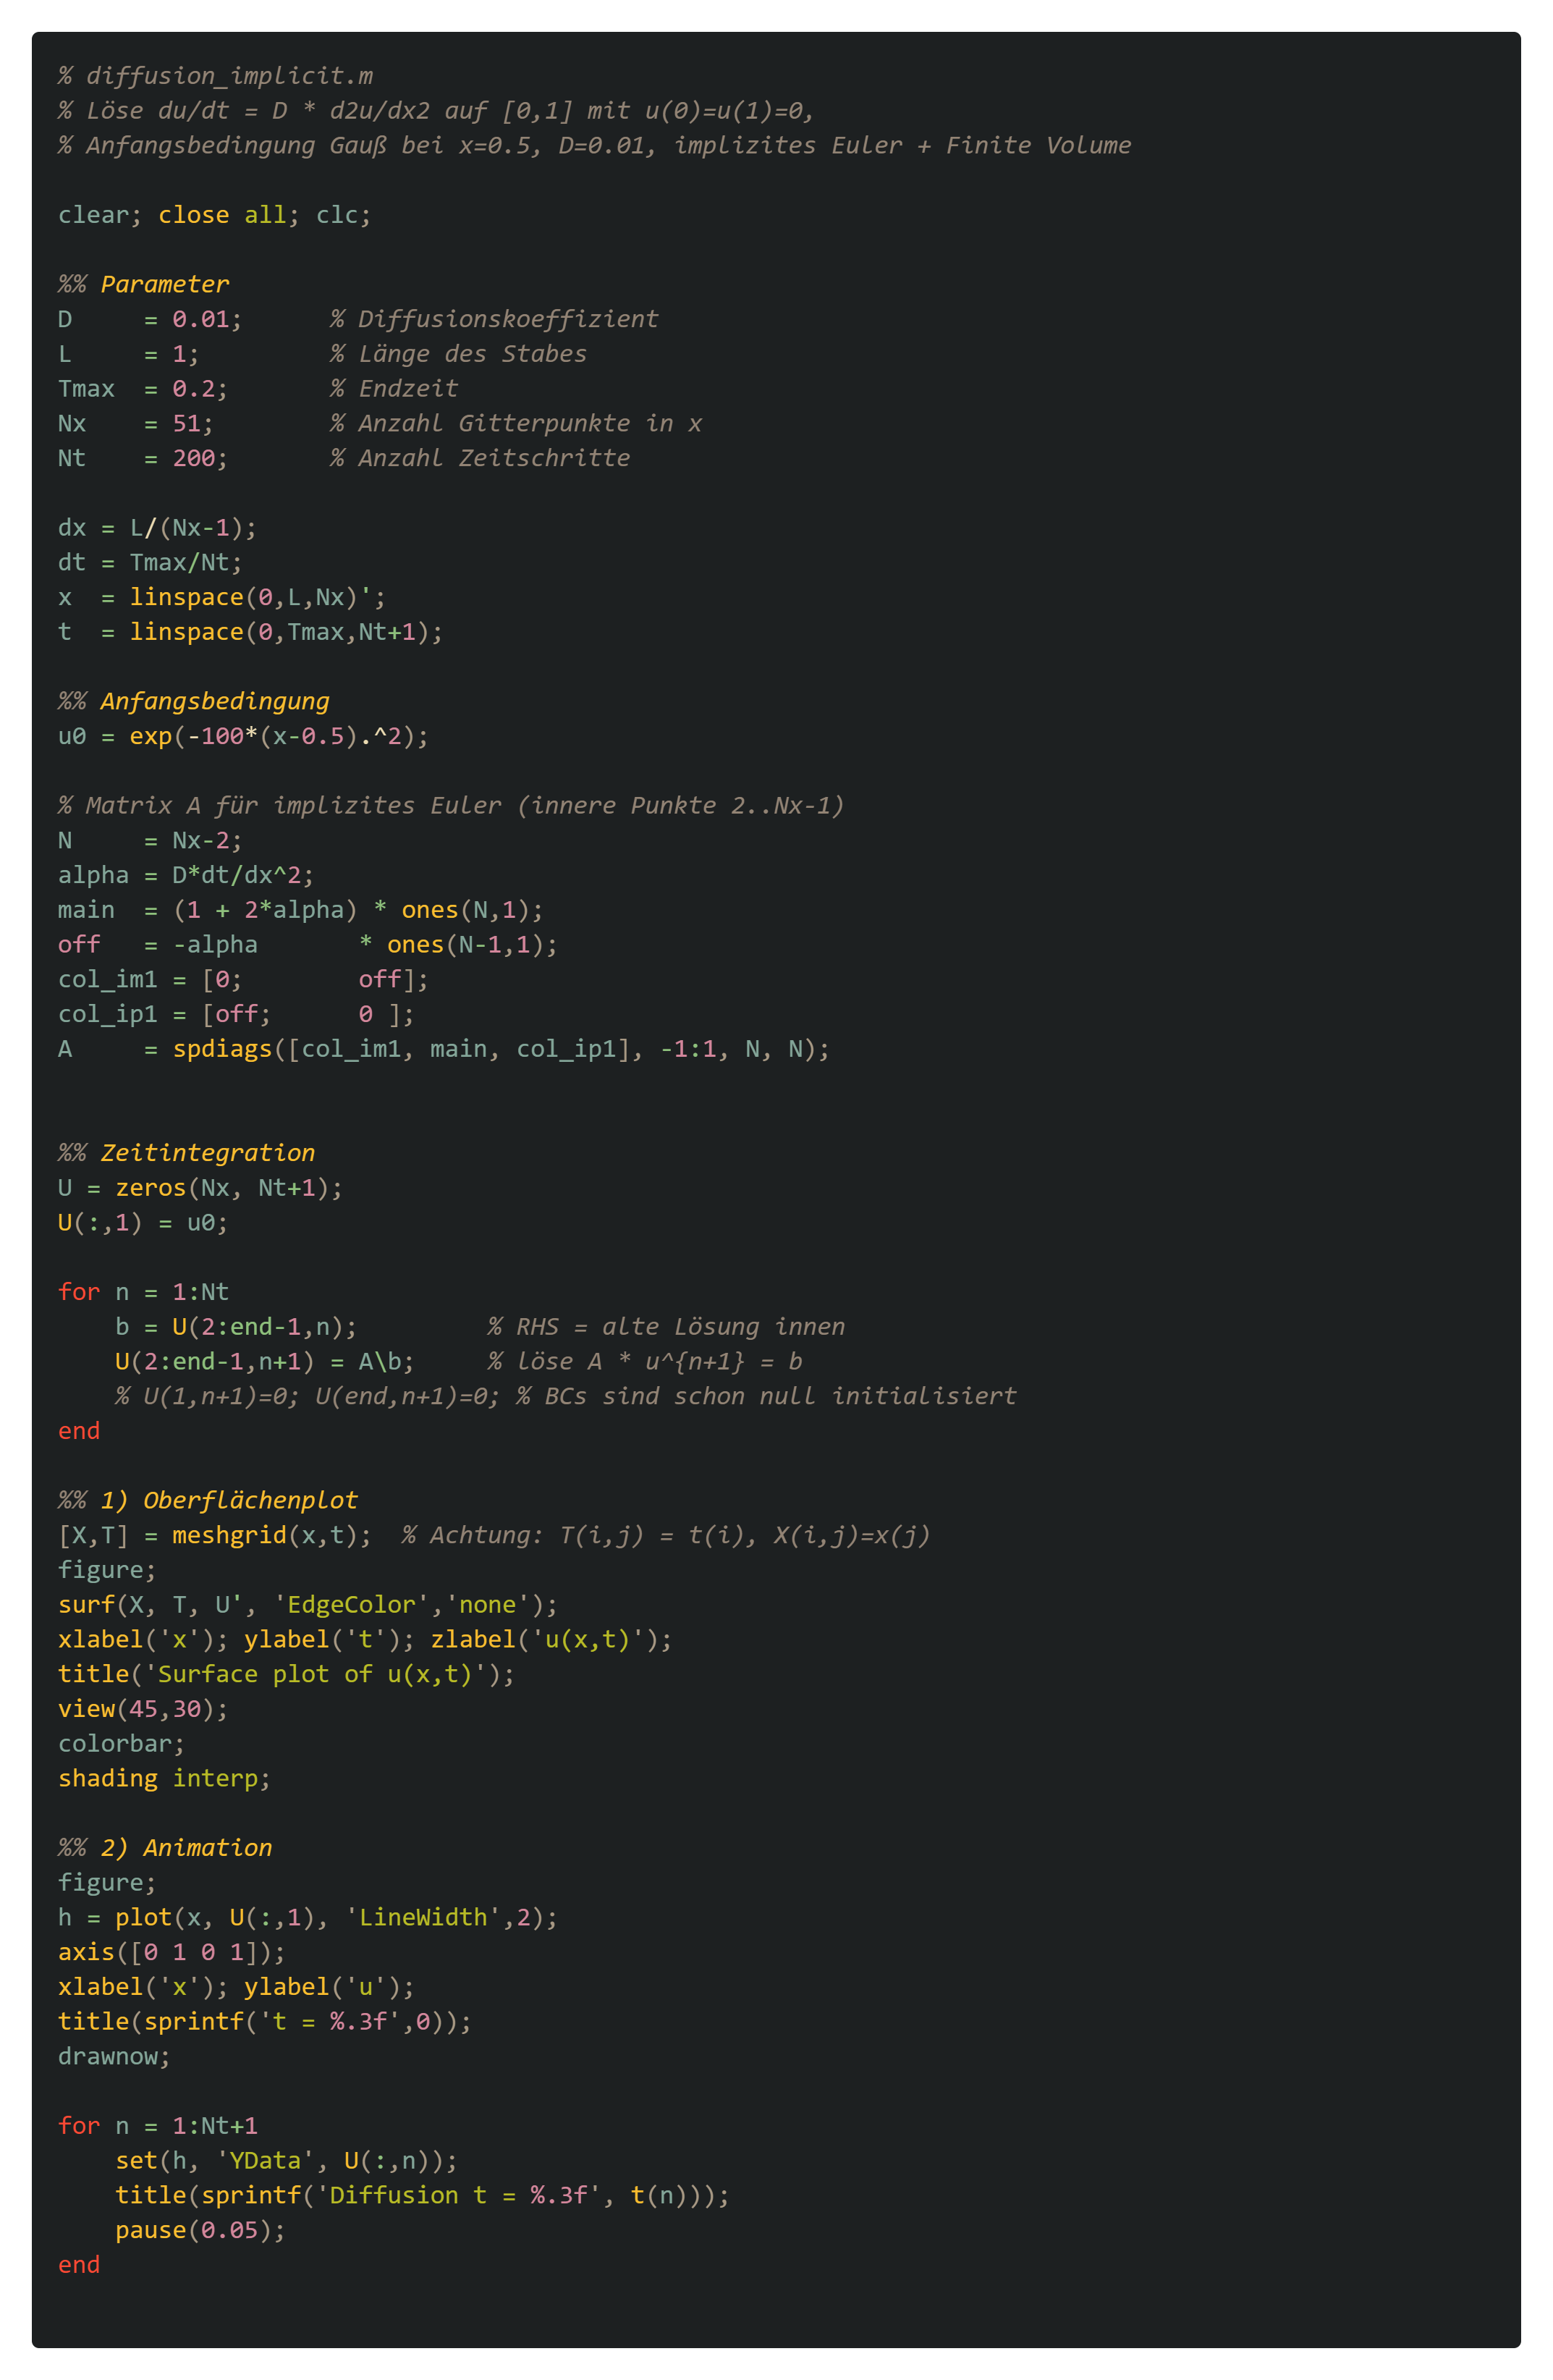
\includegraphics[scale=0.16]{HeatCode.png}
\section*{Exercise 4. Wave equation}
\subsection*{1. Command-Line Beispiel: \texttt{openExample('pde/pdedemo6')}}

Wir lösen
\[
m\,\frac{\partial^2u}{\partial t^2}
- \nabla\!\cdot(c \nabla u) + a\,u = f
\quad\text{auf }(x,y)\in[-1,1]^2
\]
mit
\[
m=1,\quad c=1,\quad a=0,\quad f=0.
\]

\subsubsection*{Randbedingungen}
\begin{itemize}
  \item \textbf{Dirichlet:} 
  \[
    u = 0
    \quad\text{auf den linken und rechten Rändern.}
  \]
  \item \textbf{Neumann:} 
  \[
    \frac{\partial u}{\partial n} = 0
    \quad\text{auf den oberen und unteren Rändern.}
  \]
\end{itemize}

\subsubsection*{Anfangsbedingungen}
\[
u(x,y,0) \;=\; \arctan\!\bigl(\cos(\tfrac{\pi}{2}x)\bigr),
\qquad
u_t(x,y,0) \;=\; 3\,\sin(\pi x)\,\exp\!\bigl(\sin(\tfrac{\pi}{2}y)\bigr).
\]

\bigskip
\subsection*{2. PDE-App Beispiel: „Wave Equation on a Square Domain“}

Das gleiche PDE und Gebiet, eingerichtet in der PDE Modeler App.

\subsubsection*{Randbedingungen}
\begin{itemize}
  \item \textbf{Dirichlet:} 
  \[
    u = 0
    \quad\text{links und rechts.}
  \]
  \item \textbf{Neumann:} 
  \[
    \frac{\partial u}{\partial n} = 0
    \quad\text{oben und unten.}
  \]
\end{itemize}

\subsubsection*{Anfangsbedingungen}
\[
u(x,y,0) = \arctan\!\bigl(\cos(\tfrac{\pi}{2}x)\bigr),
\qquad
u_t(x,y,0) = 3\,\sin(\pi x)\,\exp\!\bigl(\sin(\tfrac{\pi}{2}y)\bigr).
\]

\subsection{wave equation:}
Ich habe es nicht hinbekommen die PDE Modeler App zu benutzen.
Hier ist eine Lösung mit einem Matlab script stadtessen.
$u(0,t)=u(1,t)=0,$\\
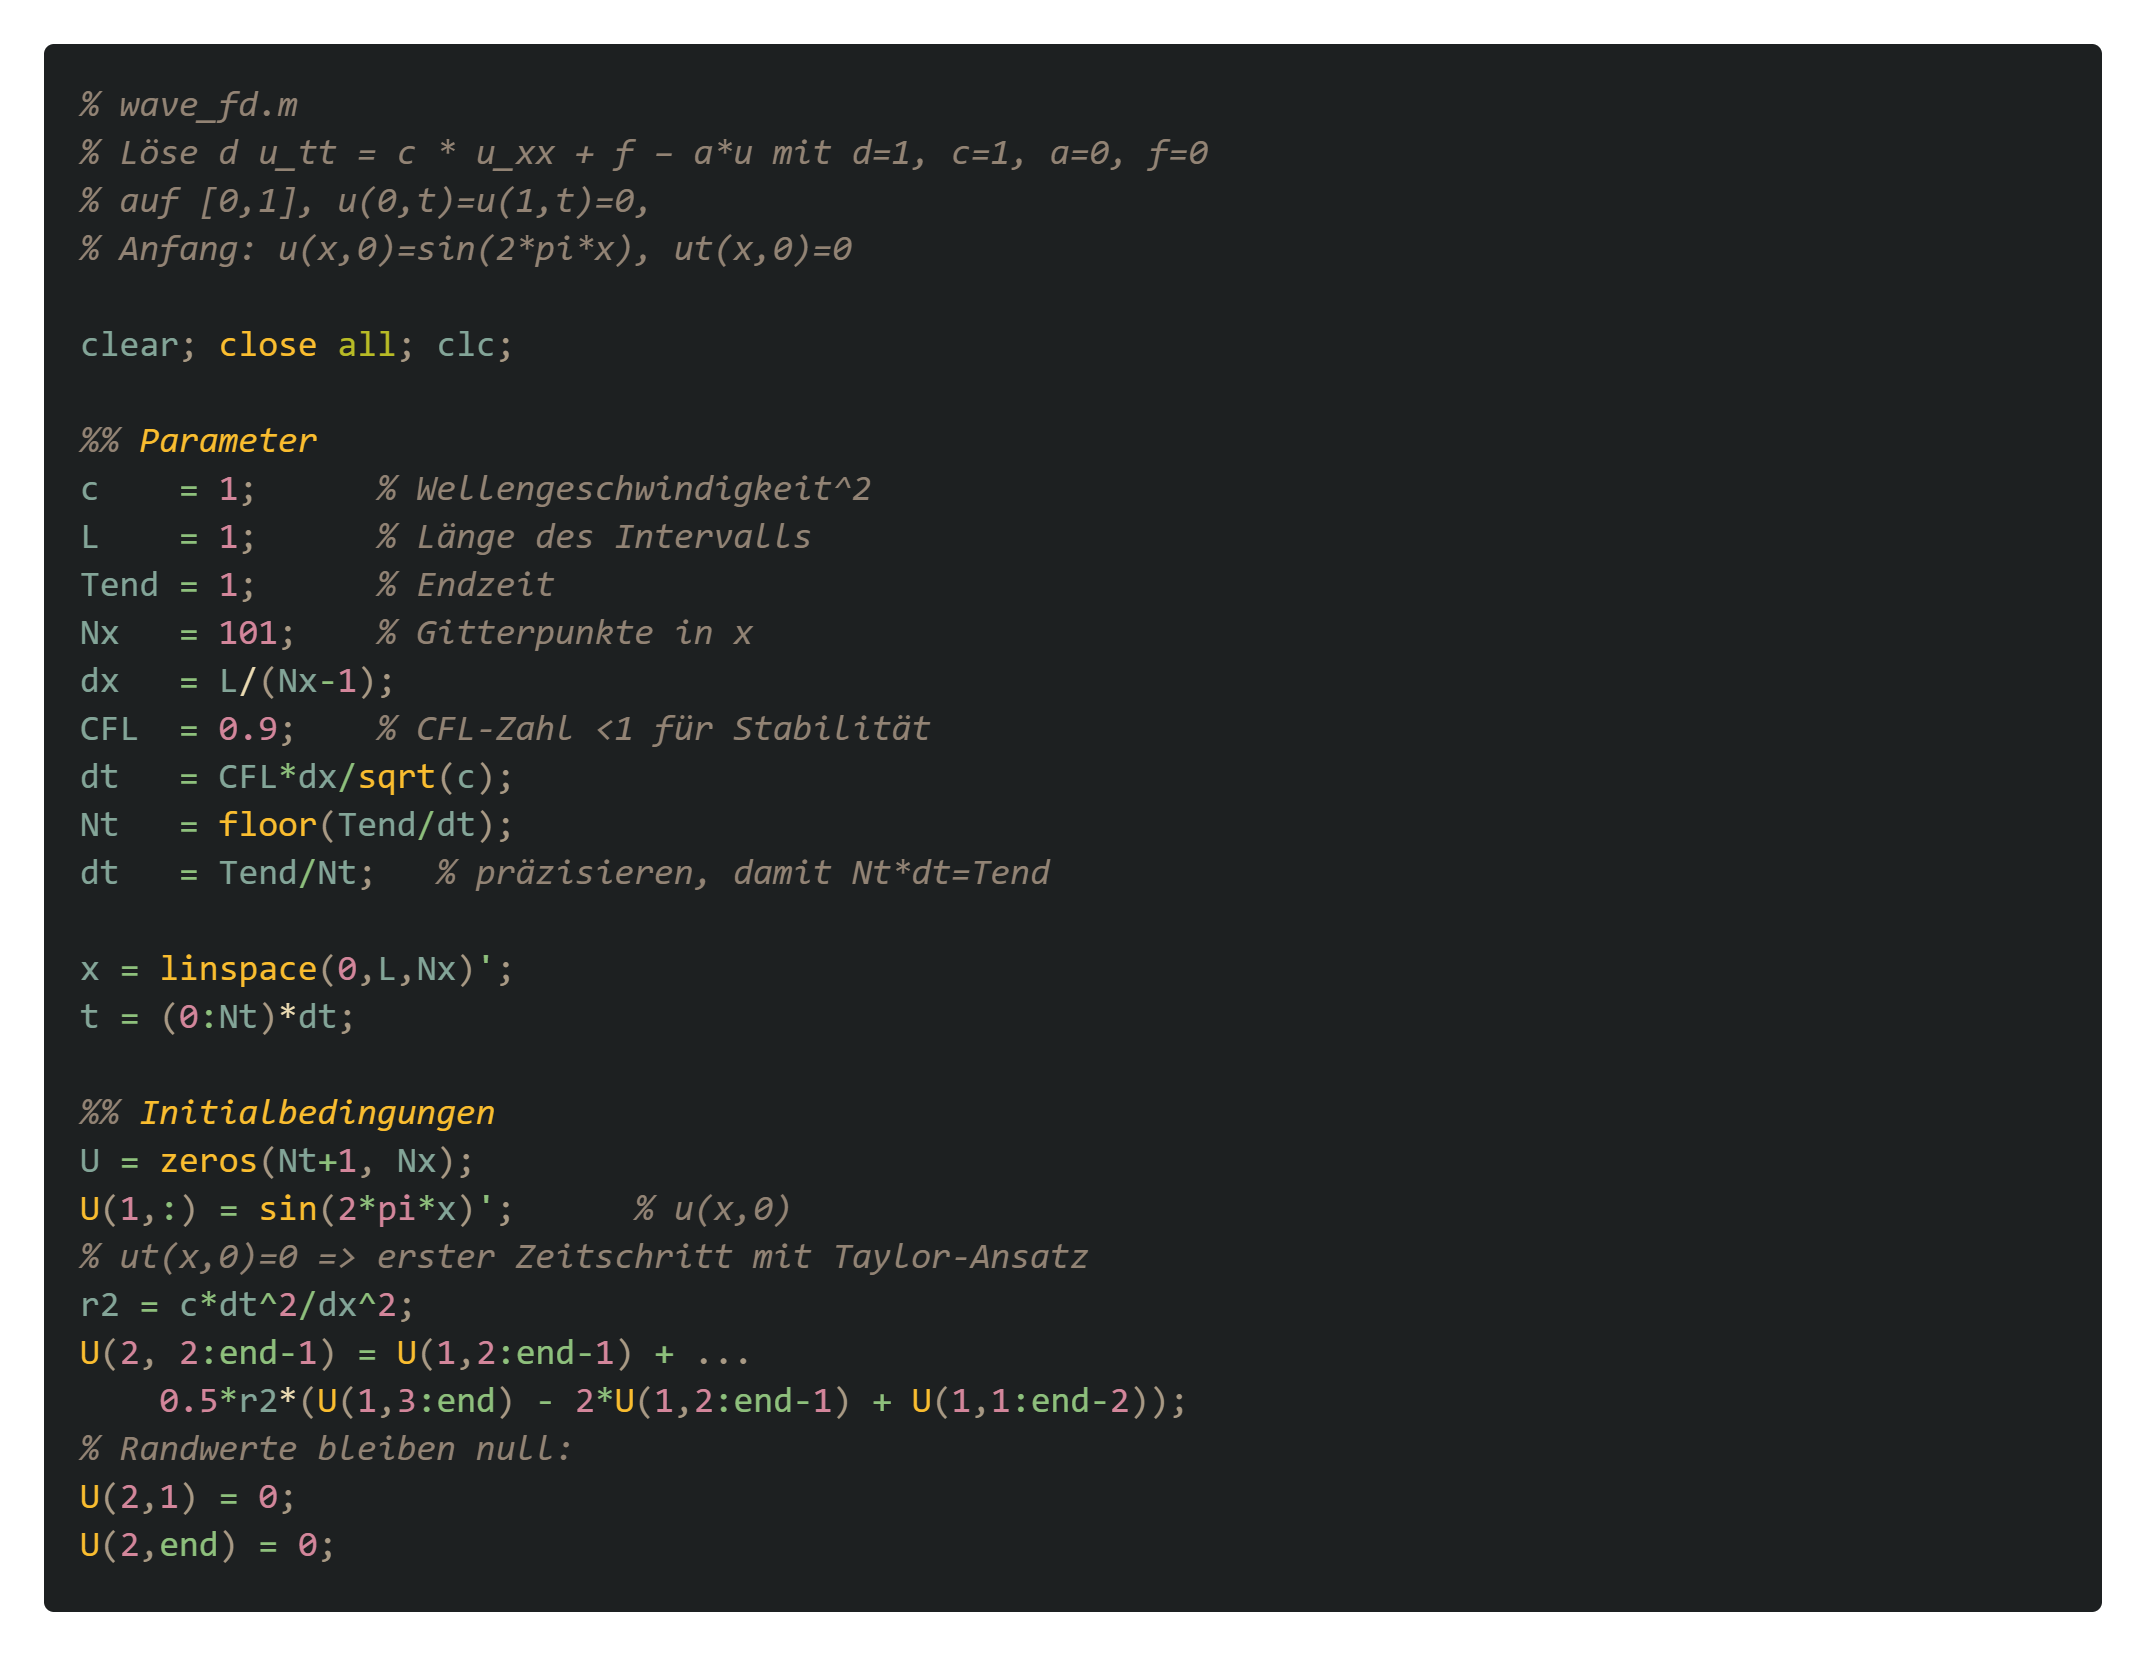
\includegraphics[scale=0.2]{WaveCode1.png}\\
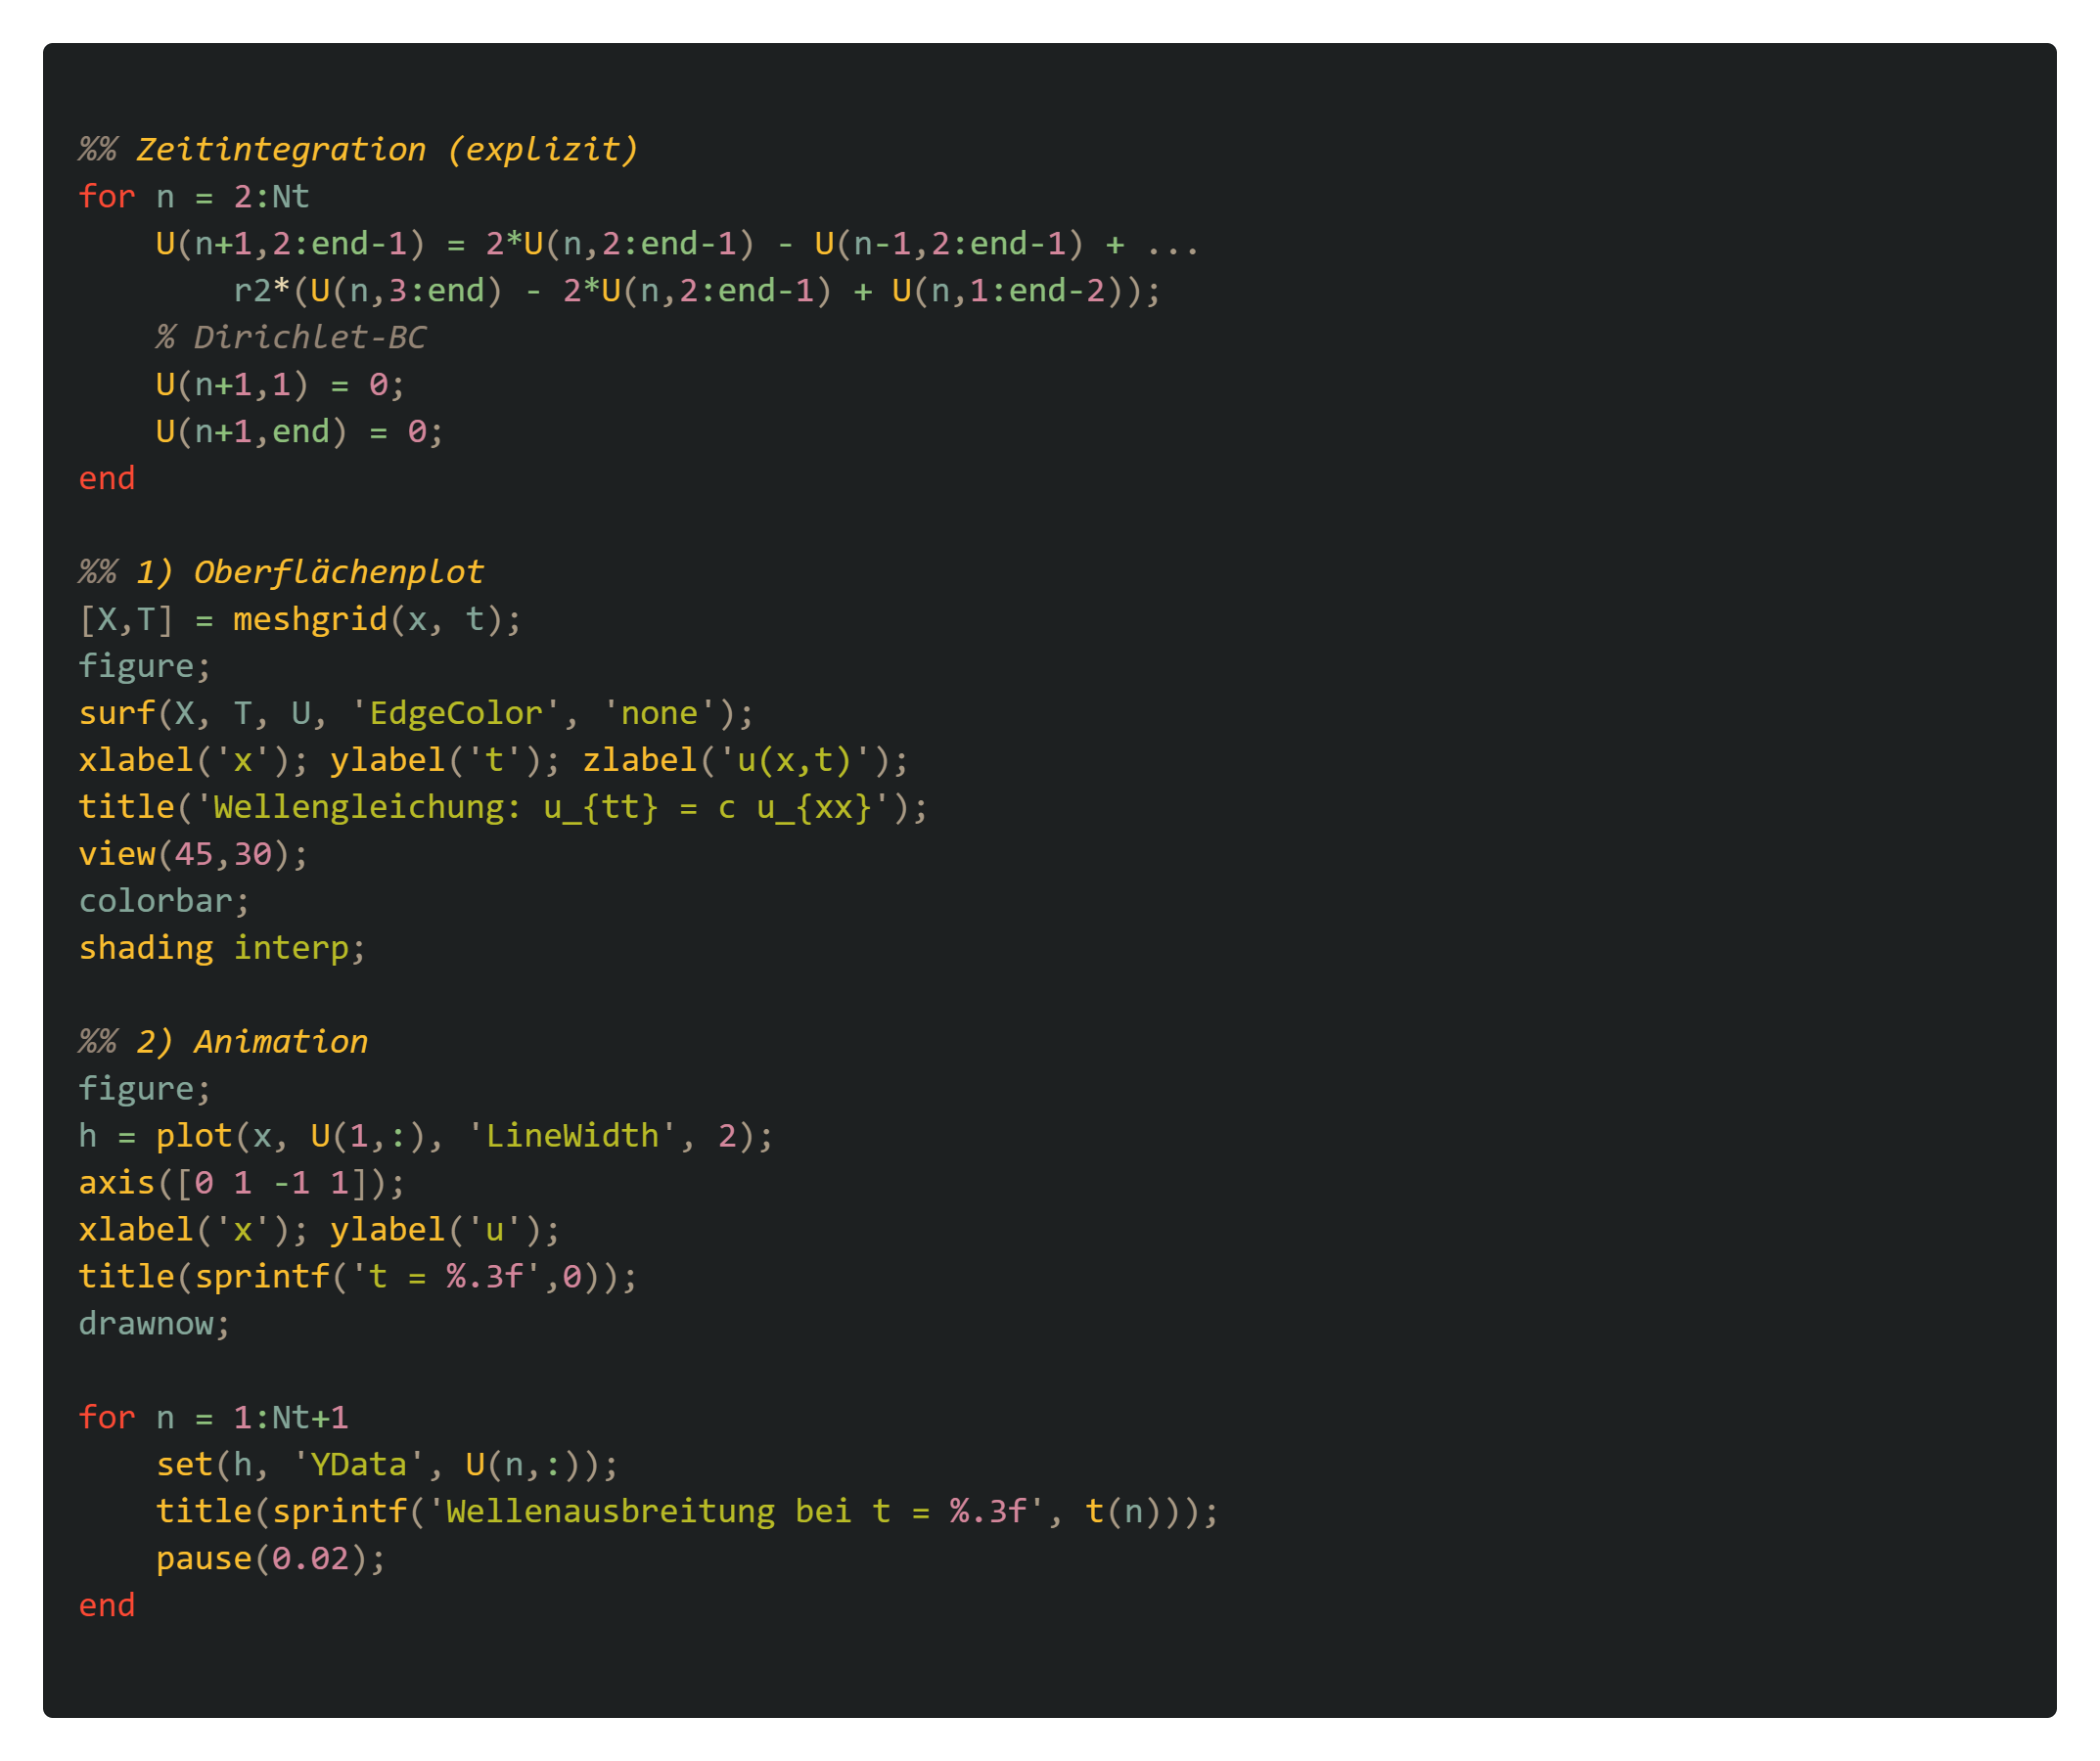
\includegraphics[scale=0.2]{WaveCode2.png}\\



\section*{\href{https://github.com/7hands/Angewandte-Modellierung-25-Colmant}{Github}}
Wie immer sind alle meine benutzten Dateien auf meinem Github zu finden.




\end{document}